\scanpage{15}
\uline{Comparaison de classes fondamentales}\quad analytiques ($=$ alg) et topologiques ($=$ transc.).

$X$ variété \deleted{\unsure{analyti}} holomorphe

$Y$ ss-variété holomorphe de codim $p$ partout.

$\underline\Omega_X^\bullet$ résolution de $\mathbf C$

\diagram{\begin{tikzcd}[row sep=large,column sep=small]
\underline H_Y^{2p}(X,\mathbf Z)\arrow[r,"i", "\text{can}" description] & \underline H_Y^{2p}(X,\mathbf Z)\otimes_{\mathbf Z}\mathbf C\arrow[r,"\sim", "\text{can}" description] & \underline H_Y^{2p}(X,\mathbf C)\arrow[r,"\sim", "\text{De Rham (i.e. can)}" description] & \underline{\underline H}_Y^{2p}(X,\underline\Omega_X^\bullet) & \\
 & & & & \underline H_Y^p(X,\underline\Omega_X^p)\arrow[ul,"\text{suite spectrale}"]\\
\mathbf Z_{\unsure{Y|\deleted{X}}}\arrow[uu,"p_{\mathrm{top}}^{\mathbf Z}"',"\sim"]\arrow[r,hook] & \mathbf C_Y\arrow[r,equal]\arrow[uu,phantom,"\deleted{\unsure{p^{\mathbf C}}}" description] & \mathbf C_Y\arrow[uu,"p_{\mathrm{top}}^{\mathbf C}"',"\sim"]\arrow[r,"\frac1{(2i\pi)^p}"'] & \mathbf C_Y\arrow[uu,"p_{\mathrm{an}}^{\mathbf C}"',"\sim"]\arrow[ur,"\uuline{\text{résidu}}"'] & \\
 & & \deleted{\unsure{\underline H_Y^p(X,\underline\Omega_X^p)}}\deleted{\arrow[uuu,"\unsure{\rotatebox{90}{$\sim$}}" description]\arrow[ur]} & &
\end{tikzcd}}
\margin{$p_{\mathrm{top}}^{\mathbf Z}:$ Poincaré topologique local}

\margin{\figure{\begin{tikzpicture}
\node[text width=5.8cm,align=left,inner sep=6pt] (n) {\uline{Poincaré analytique local} [défini par voie ess. alg.]\par\unsure{si|à} $f_1\ldots f_p$ est un syst. d'équations locales de $Y$, on prend la section $\dfrac{df_1}{f_1}\wedge\cdots\wedge\dfrac{df_p}{f_p}$ de $\underline H_Y^p(\underline\Omega_X^p)$)};
\draw[->] ($(n.north)+(-.5,.9)$) .. controls +(1,0) and +(.3,.5) .. (n.north);
\draw ($(n.north west)+(-1,0)$) .. controls +(.8,.2) and +(0,.4) .. ($(n.west)+(-.15,0)$) -- ($(n.south west)+(-.15,0)$) -- (n.south east);
\end{tikzpicture}}}

On est ramené au cas où $Y$ est réduit à un pt $a$ (prendre une \deleted{section} $X'^{n-p}$ transverse à $Y$ en un pt) et par cup-produit au cas où $X$ est de dim $1$, \unsure{disons} un disque de centre \unsure{$x$|$a$}.

[NB. à priori, \unsure{c'est acquis par ce qui précède} qu'il \unsure{le}\inserted{existe un} multiplicateur de la forme $\lambda^p$, $\lambda\in\mathbf C^*$ étant indépt de $X,Y,p$]. Alors on a

\diagram{\begin{tikzcd}[row sep=large,column sep=large]
H^1(X-a,\mathbf Z)\arrow[r]\arrow[d,phantom,"\rotatebox{90}{$\simeq$}" description] & H^1(X-a,\mathbf C)\arrow[r,"\sim"]\arrow[d,phantom,"\rotatebox{90}{$\simeq$}" description] & \underline{\underline H}^{1}(X-a,\underline\Omega_X^\bullet)\arrow[d,phantom,"\rotatebox{90}{$\simeq$}" description] & \\
H_a^2(X,\mathbf Z)\arrow[r] & H_a^2(X,\mathbf C)\arrow[r,"\sim"] & \underline{\underline H}_a^2(X,\underline\Omega_X^\bullet) & \\
\mathbf Z\arrow[u,"p_t^{\mathbf Z}"',"\sim"]\arrow[r] & \mathbf C\arrow[u,"p_t^{\mathbf C}"']\arrow[r,"\lambda"] & \mathbf C\arrow[u,"p_{\mathrm{an}}^{\mathbf C}"']\arrow[r] & H_a^1(X,\Omega_X^1)\arrow[ul,"\sim"]\quad\frac{dz}{z}
\end{tikzcd}}
\figure{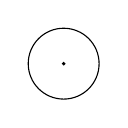
\begin{tikzpicture}\draw (0,0) circle (.45);\fill (0,0) circle (.025);\end{tikzpicture}}
\margin{14}
